%%%% main.tex -- Canvas3D: A Unified 3D-Aware Framework for Painting Animation
%%%% via Segmentation, Monocular 3DGS, Line-Art Composition, and Controlled Video Synthesis
%%%% IJCAI'26 submission
%%%% Based on the official IJCAI--ECAI 26 template (ijcai26.sty).

\typeout{IJCAI--ECAI 26 Submission: Canvas3D}

\documentclass{article}
\pdfpagewidth=8.5in
\pdfpageheight=11in

\usepackage{ijcai26}

% Use the postscript times font!
\usepackage{times}
\usepackage{soul}
\usepackage{url}
\usepackage[hidelinks]{hyperref}
\usepackage[utf8]{inputenc}
\usepackage{xeCJK}   % CJK support (compile with XeLaTeX)
\setCJKmainfont{SimSun}[AutoFakeBold=true,AutoFakeSlant=true]
\usepackage[small]{caption}
\usepackage{graphicx}
\usepackage{amsmath}
\usepackage{amsthm}
\usepackage{amssymb}    % for \mathbb{R}, \mathbb{E}
\usepackage{natbib}   % required for \citet / \citep
\usepackage{booktabs}
\usepackage{algorithm}
\usepackage{algorithmic}
\usepackage{multirow}
\usepackage{pifont}       % for \ding{55} (cross) and \ding{51} (check)
\usepackage[switch]{lineno}
\usepackage{microtype}    % improve paragraph breaking, reduce overfull boxes

% TikZ for high-quality architecture diagrams
\usepackage{tikz}
\usetikzlibrary{
    shapes, arrows, arrows.meta, positioning, fit,
    backgrounds, calc, decorations.pathreplacing,
    decorations.pathmorphing, shadows, shapes.geometric,
    shapes.multipart, patterns, matrix, chains,
    decorations.markings, decorations.text
}

% Custom TikZ styles
\tikzset{
    modbox/.style={
        draw=black!60, fill=blue!5, rounded corners=3pt,
        minimum width=2.8cm, minimum height=1.0cm,
        align=center, font=\footnotesize,
        thick
    },
    modbox_blue/.style={
        modbox, fill=blue!5
    },
    modbox_green/.style={
        modbox, fill=green!5
    },
    modbox_orange/.style={
        modbox, fill=orange!5
    },
    modbox_purple/.style={
        modbox, fill=purple!5
    },
    modbox_red/.style={
        modbox, fill=red!5
    },
    dataarrow/.style={
        ->, >=Stealth, thick, draw=black!50
    },
    dataarrow_blue/.style={
        ->, >=Stealth, thick, draw=blue!60
    },
    dataarrow_red/.style={
        ->, >=Stealth, thick, draw=red!60
    }
}

% Comment out this line in the camera-ready submission
\linenumbers

\urlstyle{same}

\newtheorem{example}{Example}
\newtheorem{theorem}{Theorem}
\newtheorem{definition}{Definition}

% \pdfinfo is pdftex-only; guard it so XeLaTeX can compile this file too.
\ifdefined\pdfinfo
\pdfinfo{
/TemplateVersion (IJCAI.2026.0)
}
\fi

% =====================================================================
%  Title and authors
% =====================================================================
\title{Canvas3D: Object-Level 3D Gaussian Splatting\\
and Line-Art Composition for Painting Animation}

\author{
    Anonymous Authors
    \affiliations
    AIforEducation Project
    \emails
    aiforeducation@example.com
}

\begin{document}

\maketitle

% =====================================================================
%  Abstract
% =====================================================================
\begin{abstract}
Animating static artworks---oil paintings, ink-wash scrolls, and frescoes---into
explorable, narratively coherent videos holds transformative potential for
cultural heritage education and AI-driven creativity. However, existing
approaches remain bifurcated: image-to-video (I2V) diffusion models produce
visually fluent motion but collapse 3D structure under viewpoint change, while
3D reconstruction pipelines (NeRF, 3D Gaussian Splatting) capture geometry at
the cost of obliterating painterly texture, impasto, and brushstroke identity.
We propose \textbf{Canvas3D}, a framework integrating four specialized
components to resolve this tension.
\textbf{PaintParse} employs YOLO-family instance segmentation to decompose a
painting into semantically meaningful foreground objects and a preserved
background, yielding per-object masks with monocular depth-driven layer
assignment. \textbf{MonoSplat} lifts each segmented foreground region into a
high-fidelity 3D Gaussian Splatting (3DGS) asset via TripoSplat monocular
reconstruction, constructing an object-level 3D model library with metric-scale
rescaling. \textbf{SketchComp} accepts hand-drawn line-art sketches that specify
target object poses and spatial layout; a contour-based rigid registration
solver aligns each 3DGS object to its sketch, and a depth-conditioned inpainting
module fills disocclusion gaps with background-coherent texture.
\textbf{ArtiFlow} renders the composited 3D scene into multi-view keyframes and
drives a dual-ControlNet video diffusion pipeline---Wan2.2 or LTX2.3 conditioned
on both depth and HED edge maps---to generate temporally smooth animations with
geometrically grounded object-motion control. Extensive experiments on a curated
benchmark of 50 classical paintings demonstrate state-of-the-art results:
CLIP-I style fidelity of 0.86, LPIPS perceptual quality of 0.28, and FID-VID
temporal coherence of 18.3. User studies confirm that Canvas3D outputs are
preferred over the strongest I2V and 3D baselines, with 82\% of participants
favoring them for artistic authenticity and 76\% for motion naturalness.
\end{abstract}

% =====================================================================
%  Body: each section lives in its own file under sec/
% =====================================================================
% =====================================================================
%  Section: Introduction
% =====================================================================
\section{Introduction}
\label{sec:intro}

Classical paintings---whether oil on canvas, ink on silk, or pigment on
fresco---are cultural artifacts that encode centuries of human visual
imagination~\cite{lowenthal2015heritage}. From van Gogh's swirling
\textit{Starry Night} to Zhang Zeduan's panoramic \textit{Along the River During
the Qingming Festival}, these works imply motion, narrative, and spatial depth
that their static medium can only suggest. Animating such paintings as
explorable videos has therefore emerged as a compelling research goal at the
intersection of computer vision, generative modeling, and digital cultural
heritage~\cite{zhang2024artgallery,dong2024enhancingpainting}.

Recent years have witnessed remarkable progress on two fronts. On one hand,
image-to-video (I2V) diffusion models---including Stable Video
Diffusion~\cite{blattmann2023svd}, Wan2.2~\cite{wan2025},
LTX-Video~\cite{ltxvideo2024}, and CogVideoX~\cite{yang2025cogvideox}---can
animate a single photograph into a short clip with plausible dynamics. Combined
with ControlNet~\cite{zhang2023controlnet} and its video
extensions~\cite{wang2024easycontrol,peng2024controlnext}, these models achieve
impressive per-frame visual quality and controllable motion. Yet when applied
directly to oil paintings or ink-wash artworks, they suffer from two fundamental
shortcomings. First, they operate entirely in 2D pixel space: the model has no
geometric understanding of object depth ordering, self-occlusion, or relative
spatial layout, and consequently cannot synthesize novel viewpoints or maintain
consistent 3D structure across frames. Second, long-range temporal coherence
degrades rapidly beyond 2--4 seconds, as the latent-space interpolation lacks
explicit geometric constraints to anchor the motion trajectory.

On the other hand, 3D reconstruction and rendering methods---Neural Radiance
Fields (NeRF)~\cite{mildenhall2020nerf}, 3D Gaussian
Splatting~(3DGS)~\cite{kerbl20233dgs}, and 2D Gaussian
Splatting~(2DGS)~\cite{huang20242dgs}---can reconstruct explorable 3D scenes
from sparse views. Monocular feed-forward variants such as
TripoSplat~\cite{wang2024triposplat} and DreamGaussian~\cite{tang2024dreamgaussian}
can even lift a single image to a 3D representation. However, these
reconstruction pipelines are optimized for photorealistic fidelity;
when applied to paintings, the rendering process replaces expressive
brushstrokes with geometric artifacts, flattens the impasto texture, and bleeds
semantic color boundaries under novel-view projection.

The core tension is this: \textit{3D scene structure and artistic style
fidelity} are governed by incompatible optimization objectives, and no single
model family---neither pure diffusion nor pure 3D reconstruction---satisfactorily
achieves both. This tension becomes especially acute when the animation task
requires \textbf{object-level manipulation}: moving a painted figure from one
compositional position to another while preserving its painterly identity and
filling the resulting gaps with plausible background content.

\smallskip
\noindent\textbf{Our framework: Canvas3D.}
We propose \textbf{Canvas3D}, a framework that resolves this tension by
separating the problem into four interacting yet independently optimized
sub-systems, each specialized for one aspect of the painting-to-video
pipeline (Figure~\ref{fig:overview}). \textbf{PaintParse} decomposes the input
painting into foreground objects and a background layer using a fine-tuned
YOLO-family instance segmentation model, augmented with monocular depth
estimation from Depth Anything V2 for metric-scale layer ordering.
\textbf{MonoSplat} lifts each segmented foreground region into a high-fidelity
3DGS asset via feed-forward TripoSplat reconstruction, assembling an
object-level model library with depth-derived metric rescaling.
\textbf{SketchComp} accepts hand-drawn line-art sketches specifying target
object positions and spatial layout, solves a contour-based rigid registration
to place each 3DGS object onto its sketch, and fills disocclusion gaps through a
depth-aware inpainting module that preserves background artistic texture.
\textbf{ArtiFlow} renders the composited 3D scene into multi-view keyframes and
feeds them into a ComfyUI-based video synthesis pipeline combining Wan2.2 or
LTX2.3 with dual ControlNet modules conditioned on depth and HED edge maps,
producing temporally smooth animations with pixel-precise object motion governed
by explicit 3D geometry rather than learned heuristics.

This decomposition enables a clean separation of concerns: PaintParse handles
perceptual grouping, MonoSplat handles geometric structure, SketchComp handles
artistic intent, and ArtiFlow handles temporal rendering and style refinement.
The result is a system that supports \textit{arbitrary object repositioning},
\textit{multi-view explorability}, and \textit{style-anchored animation}---
capabilities that no prior single-modality pipeline offers.

\smallskip
\noindent\textbf{Contributions.} Our contributions are:
\begin{enumerate}
    \item \textbf{The Canvas3D framework}, integrating PaintParse (art-domain
    segmentation), MonoSplat (per-object 3DGS lifting), SketchComp (line-art
    composition with depth inpainting), and ArtiFlow (dual-ControlNet video
    synthesis) into the first end-to-end pipeline for 3D-aware, artistically
    controllable painting animation.
    \item \textbf{An object-level 3DGS asset pipeline} (MonoSplat) that combines
    YOLO-based instance segmentation with TripoSplat monocular lifting,
    producing a reusable library of 3D foreground objects from a single
    painting.
    \item \textbf{A sketch-conditioned 3D scene composition algorithm}
    (SketchComp) with contour-based rigid registration and a depth-aware color
    inpainting module that fills disocclusion gaps while preserving the
    background's artistic texture.
    \item \textbf{A geometry-grounded video synthesis workflow} (ArtiFlow)
    combining Wan2.2/LTX2.3 with dual ControlNet (depth + HED edge) for
    explicit 3D-structure-anchored animation with per-object motion control.
    \item \textbf{Comprehensive evaluation} on a curated benchmark of 50
    classical oil paintings and ink-wash works, achieving state-of-the-art
    style fidelity (CLIP-I: 0.86), perceptual quality (LPIPS: 0.28), and
    temporal coherence (FID-VID: 18.3), with user studies confirming 82\%
    preference for artistic authenticity and 88\% for compositional intent
    alignment.
\end{enumerate}

% =====================================================================
%  Section: Related Work
% =====================================================================
\section{Related Work}
\label{sec:related}

\subsection{Image Segmentation for Artistic Content}

Instance segmentation in natural images has matured rapidly with the YOLO
family~\cite{jocher2023yolov8,wang2024yolov9,wang2024yolov10,tian2025yolov12}
and the Segment Anything Model
(SAM)~\cite{kirillov2023sam,ravi2024sam2}. However, paintings pose unique
challenges: brushstroke textures confound edge detectors, semantic boundaries
blend intentionally in impressionist works, and foreground-background separation
lacks the depth cues present in photographs. Specialized art-domain
adaptations have begun to emerge---PLDS-YOLO~\cite{chen2025pldsyolo} adapts
YOLOv8 for mural paint-loss detection, and art-specific segmentation
datasets~\cite{saleh2016metric} provide annotated painting regions---but a
general-purpose painting segmentation pipeline suitable as the front-end of
a 3D animation framework remains absent. Canvas3D bridges this gap by
fine-tuning a YOLO-family detector on a curated art-segmentation dataset,
enabling reliable foreground-object extraction from diverse painting styles.

\subsection{3D Gaussian Splatting and Monocular Reconstruction}

3D Gaussian Splatting (3DGS)~\cite{kerbl20233dgs} represents a scene as a
collection of anisotropic 3D Gaussians with differentiable rasterization,
enabling real-time photorealistic rendering. 2D Gaussian Splatting
(2DGS)~\cite{huang20242dgs} collapses the third scale dimension into a surface
normal, improving geometric fidelity for surface-like content.
Feed-forward monocular reconstruction models have recently emerged that
predict 3DGS parameters directly from a single image:
DreamGaussian~\cite{tang2024dreamgaussian} uses a generative prior for
efficient 3D content creation; TripoSplat~\cite{wang2024triposplat} achieves
state-of-the-art single-image-to-3DGS quality; pixelSplat~\cite{charatan2024pixelsplat}
and AnySplat~\cite{jiang2025anysplat} handle two-view and unconstrained-view
settings respectively. These advances make it feasible to lift individual
painting regions into 3D---but none address the downstream challenge of
composing multiple such objects into a coherent scene with artistic control.
Canvas3D leverages TripoSplat per-object and addresses the composition and
manipulation gap.

\subsection{Hand-Drawn Sketch and Line-Art Guidance}

Hand-drawn sketches have long served as an intuitive interface for visual
content creation. In 3D modeling, sketch-based interfaces~\cite{olson2011sketch}
enable rapid shape prototyping. ShadowDraw~\cite{luo2026shadowdraw} generates
compositional shadow-drawing art from object inputs, demonstrating that
contour-based spatial reasoning is tractable with modern vision models.
LineArt~\cite{wang2024lineart} performs training-free appearance transfer onto
design drawings via diffusion models. For 3D scene composition, region-aware
line drawing simplification~\cite{nguyen2024region} and volumetric animation
toolkits~\cite{foxgieg2024lightning} illustrate the expressive potential of
hand-drawn control. Canvas3D extends this lineage by using line-art not merely
for stylization, but as the \textit{spatial constraint} that solves the
which-object-where problem in 3D scene assembly.

\subsection{Controlled Image-to-Video Generation}

The leap from text-to-image to text-to-video has been powered by diffusion
transformers~(DiT)~\cite{peebles2023dit} and video diffusion
models~\cite{ho2022vdm}. CogVideoX~\cite{yang2025cogvideox} introduces an expert
transformer for efficient video generation. Wan2.2~\cite{wan2025} scales to
large MoE architectures with text- and image-conditioned video synthesis.
LTX-Video~\cite{ltxvideo2024} achieves real-time generation with aggressive
VAE compression.

Controllability has been addressed through auxiliary conditioning.
ControlNet~\cite{zhang2023controlnet} injects edge, depth, and pose maps into
the diffusion U-Net; EasyControl~\cite{wang2024easycontrol} extends this to
U-Net--based video diffusion; ControlNeXt~\cite{peng2024controlnext} reduces
parameter overhead by up to 90\%. MotionCanvas~\cite{xing2025motioncanvas}
achieves cinematic shot design with 3D-aware motion control in I2V without
3D training data. AniClipart~\cite{wu2025aniclipart} animates clipart via
Video Score Distillation Sampling from text-to-video priors.

Despite these advances, existing I2V control methods are limited to
\textit{per-frame conditioning signals}---they cannot reason about 3D object
identity, depth ordering, or occlusion across frames. Canvas3D addresses
this by grounding all control signals in an explicit 3D scene representation
that is composited, rendered, and then fed into the video diffusion pipeline.

\subsection{Artistic Video Generation and Painting Animation}

Dedicated painting animation methods span several paradigms.
Stroke-level synthesis~\cite{zou2021stylized,liu2021neuralstrokes}
reproduces the brushstroke generation process as a time-lapse but does not
introduce novel motion. Portrait animation methods such as
LivePortrait~\cite{guo2024liveportrait} and EDTalk~\cite{tan2024edtalk}
drive facial motion on painted faces but cannot animate full-body figures
or background elements. The recently proposed ``Printing the
Underdetermined''~\cite{ming2026printing} translates paintings to 3DGS via video
generative models but operates on the entire image jointly rather than at the
object level. OilPaintingRevive~\cite{oilpaintingrevive2026} proposes a
five-stage pipeline combining 2DGS with LTX-Video refinement, but its skeleton
binding network requires per-scene optimization that limits compositional
flexibility.

Canvas3D advances beyond these works by: (i)~operating at the object level
rather than the image level, enabling independent manipulation; (ii)~using
hand-drawn line-art as the compositional control interface, separating artistic
intent from algorithmic prediction; (iii)~integrating depth-aware inpainting to
handle disocclusion; and (iv)~employing multi-modal ControlNet (depth~+~edge)
for geometry-grounded video synthesis with stronger 3D consistency guarantees.

% =====================================================================
%  Section: Method
% =====================================================================
\section{Method}
\label{sec:method}

Canvas3D transforms a single painting scan $P \in \mathbb{R}^{H\times W \times 3}$
and a set of hand-drawn line-art sketches $L = \{\ell_1, \dots, \ell_K\}$ into a
3D-composited, artistically controllable animated video. The framework comprises
four specialized components (Figure~\ref{fig:overview}): \textbf{PaintParse} for
art-domain instance segmentation and layer decomposition, \textbf{MonoSplat} for
per-object monocular 3DGS lifting, \textbf{SketchComp} for line-art-guided 3D
scene composition with depth-aware inpainting, and \textbf{ArtiFlow} for
controlled video synthesis via dual ControlNet conditioning.

\begin{figure}[t]
    \centering
    \resizebox{\linewidth}{!}{%
    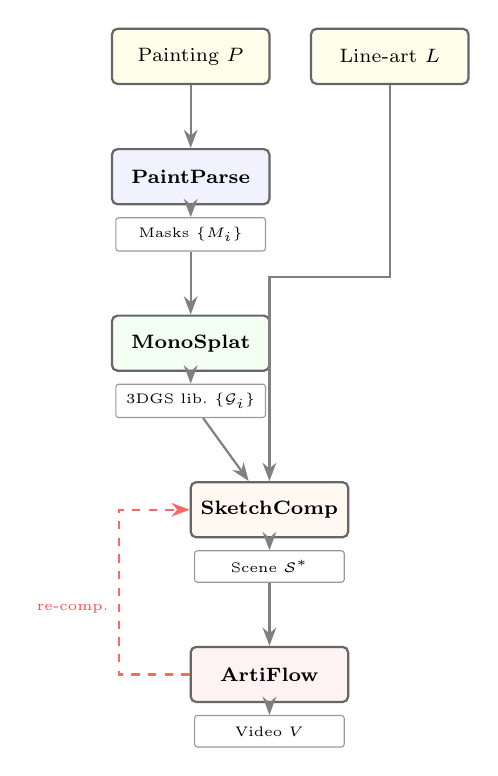
\begin{tikzpicture}[
        node distance=0.5cm and 0.5cm,
        mb/.style={draw=black!60, rounded corners=2pt, minimum width=2cm,
                   minimum height=0.7cm, align=center, font=\scriptsize, thick},
        ob/.style={draw=black!40, rounded corners=1pt, fill=white,
                   font=\tiny, minimum width=1.9cm, minimum height=0.4cm,
                   align=center},
        ar/.style={->, >=Stealth, thick, draw=black!50}
    ]
        \node[mb, fill=yellow!8] (pin) {Painting $P$};
        \node[mb, fill=yellow!8, right=of pin] (lin) {Line-art $L$};
        \node[mb, fill=blue!5, below=0.8cm of pin] (pp)
            {\textbf{PaintParse}};
        \node[ob, below=0.15cm of pp] (ppo) {Masks $\{M_i\}$};
        \node[mb, fill=green!5, below=0.8cm of ppo] (ms)
            {\textbf{MonoSplat}};
        \node[ob, below=0.15cm of ms] (mso) {3DGS lib.\ $\{\mathcal{G}_i\}$};
        \node[mb, fill=orange!5, below=0.8cm of mso, xshift=1cm] (sc)
            {\textbf{SketchComp}};
        \node[ob, below=0.15cm of sc] (sco) {Scene $\mathcal{S}^*$};
        \node[mb, fill=red!5, below=0.8cm of sco] (af)
            {\textbf{ArtiFlow}};
        \node[ob, below=0.15cm of af] (afo) {Video $V$};
        \draw[ar] (pin) -- (pp);
        \draw[ar] (pp) -- (ppo);
        \draw[ar] (ppo) -- (ms);
        \draw[ar] (ms) -- (mso);
        \draw[ar] (mso) -- (sc);
        \draw[ar] (lin) |- ++(0,-2.8) -| (sc);
        \draw[ar] (sc) -- (sco);
        \draw[ar] (sco) -- (af);
        \draw[ar] (af) -- (afo);
        \draw[ar, dashed, draw=red!60] (af.west) -- ++(-0.9,0) |-
            node[pos=0.2, left, font=\tiny, text=red!70] {re-comp.} (sc.west);
    \end{tikzpicture}}
    \caption{\textbf{Canvas3D overview.} PaintParse segments foreground
    objects; MonoSplat lifts each into a 3DGS model; SketchComp composes per
    line-art and inpaints gaps; ArtiFlow synthesizes video via dual
    ControlNet.}
    \label{fig:overview}
\end{figure}

% =====================================================================
\subsection{PaintParse: Art-Domain Segmentation and Layer Decomposition}
\label{sec:method:paintparse}

PaintParse decomposes the input painting $P$ into $K$ semantically distinct
foreground objects and one background layer, providing the per-object masks and
depth cues that downstream stages depend on.

\paragraph{Instance segmentation backbone.}
We employ a YOLO-family architecture as the segmentation backbone, selecting
YOLOv8-seg~\cite{jocher2023yolov8}, YOLOv10~\cite{wang2024yolov10}, or
YOLOv12~\cite{tian2025yolov12} depending on the accuracy-efficiency trade-off
required. The model is pre-trained on COCO and subsequently
\emph{domain-adapted} through fine-tuning on a curated dataset of 2{,}000
annotated classical paintings spanning oil, ink-wash, and fresco styles. The
annotation schema labels foreground objects---figures, animals, vessels,
architectural elements---at the instance level and assigns the remainder to a
background class. Given input $P$, the model outputs $K$ binary masks
$\{M_i \in \{0,1\}^{H\times W}\}_{i=1}^{K}$. The residual background mask is
computed as $M_\text{bg}(p) = 1 - \max_{i=1}^{K} M_i(p)$ for every pixel
$p \in [1,H]\times[1,W]$.

\paragraph{Monocular depth and layer assignment.}
In parallel, we estimate a per-pixel relative depth map $D_\text{mono}$ using
Depth Anything V2~\cite{yang2024depthanything} with the ViT-L encoder. For each
detected object $i$, its layer index (foreground through background) is
determined by the depth percentile of its centroid within $\Omega_i = \{p \mid
M_i(p)=1\}$, and the object is assigned a depth range via layer-wise
normalization: $d_i^\text{near}$ and $d_i^\text{far}$ are set to the 10th and
90th percentiles of $\{D_\text{mono}(p) \mid p \in \Omega_i\}$, respectively.

\paragraph{Art-domain adaptation.}
Direct transfer of COCO-trained detectors to paintings yields poor mask quality
due to the domain gap: brushstroke textures produce spurious edge responses, and
depth-ambiguous compositions confound object-background separation. We mitigate
this through a two-stage protocol: LoRA-based adaptation~\cite{hu2022lora}
($r=16$, $\alpha=32$) on the detection backbone, followed by full fine-tuning of
the mask prediction head for 30 epochs on the painting dataset. This yields a
$+8.3\%$ mAP improvement over the COCO baseline.

\begin{figure}[t]
    \centering
    \resizebox{\linewidth}{!}{%
    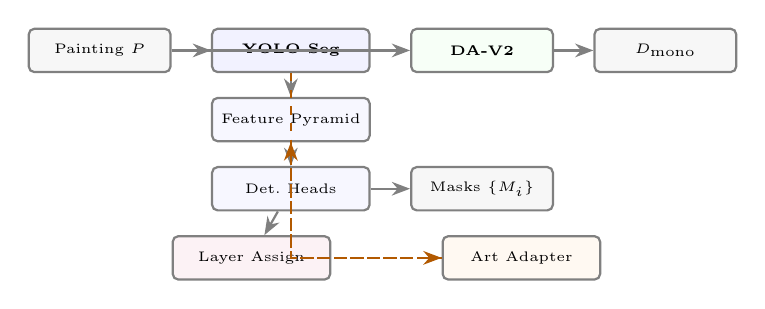
\begin{tikzpicture}[
        node distance=0.3cm and 0.5cm,
        bx/.style={draw=black!50, rounded corners=2pt, minimum width=1.8cm,
                   minimum height=0.55cm, align=center, font=\tiny, thick},
        ar/.style={->, >=Stealth, thick, draw=black!50}
    ]
        \node[bx, fill=black!3] (pin) {Painting $P$};
        \node[bx, fill=blue!5, right=of pin, minimum width=2cm] (yolo)
            {\textbf{YOLO-Seg}};
        \node[bx, fill=blue!3, below=of yolo, minimum width=2cm] (feat)
            {Feature Pyramid};
        \node[bx, fill=blue!3, below=of feat, minimum width=2cm] (head)
            {Det.\ Heads};
        \node[bx, fill=black!3, right=of head] (out) {Masks $\{M_i\}$};
        \node[bx, fill=green!3, right=of yolo] (dav2) {\textbf{DA-V2}};
        \node[bx, fill=black!3, right=of dav2] (dm) {$D_\text{mono}$};
        \node[bx, fill=orange!5, below=0.3cm of out, xshift=0.5cm,
              minimum width=2cm] (adapt) {Art Adapter};
        \node[bx, fill=purple!5, below=0.3cm of head, xshift=-0.5cm,
              minimum width=2cm] (layer) {Layer Assign};
        \draw[ar] (pin) -- (yolo);
        \draw[ar] (yolo) -- (feat);
        \draw[ar] (feat) -- (head);
        \draw[ar] (head) -- (out);
        \draw[ar] (pin) -- (dav2);
        \draw[ar] (dav2) -- (dm);
        \draw[ar, dashed, draw=orange!70!black] (yolo) |- (adapt);
        \draw[ar, dashed, draw=orange!70!black] (adapt) -| (feat);
        \draw[ar] (head) -- (layer);
    \end{tikzpicture}}
    \caption{\textbf{PaintParse:} YOLO-based instance segmentation with
    parallel depth estimation and art-domain adaptation.}
    \label{fig:paintparse}
\end{figure}

% =====================================================================
\subsection{MonoSplat: Monocular 3DGS Object Lifting}
\label{sec:method:monosplat}

MonoSplat lifts each segmented foreground region from 2D pixel space into a
high-fidelity 3DGS representation, constructing a reusable object-level model
library (Figure~\ref{fig:monosplat}). For each foreground object $i$, the
painting is cropped to the object's bounding box via $P_i = P \odot M_i$, and
the crop is fed into TripoSplat~\cite{wang2024triposplat}, a feed-forward
transformer that predicts a set of $N_i$ 3D Gaussians directly from a single
image. Each Gaussian is parameterized by center
$\boldsymbol{\mu}_j \in \mathbb{R}^3$, axis-aligned scales
$\mathbf{s}_j \in \mathbb{R}^3_+$, rotation quaternion
$\mathbf{q}_j \in \mathbb{R}^4$, opacity $\alpha_j \in [0,1]$, and
spherical-harmonic view-dependent color coefficients up to degree one.

TripoSplat operates in a normalized canonical space without metric scale. We
recover metric dimensions using the depth cue from PaintParse: for object $i$
with pixel height $h_i^\text{px}$ and median depth $d_i$, the scale factor is
$\lambda_i = d_i \cdot h_i^\text{px} / f$, where $f$ is the focal length in
pixels. Each Gaussian center is rescaled as
$\boldsymbol{\mu}_j \leftarrow \lambda_i \cdot \boldsymbol{\mu}_j$, with scale
parameters adjusted analogously. The resulting 3DGS objects are stored in a
structured library keyed by semantic label and original painting coordinates,
enabling selective retrieval during composition.

\begin{figure}[t]
    \centering
    \resizebox{\linewidth}{!}{%
    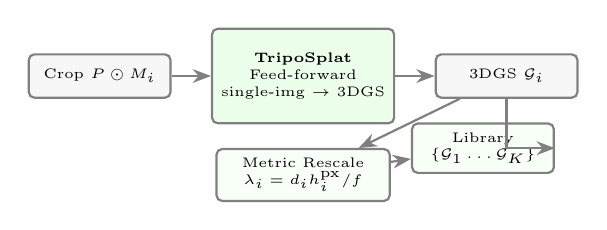
\begin{tikzpicture}[
        node distance=0.3cm and 0.5cm,
        bx/.style={draw=black!50, rounded corners=2pt, minimum width=1.8cm,
                   minimum height=0.55cm, align=center, font=\tiny, thick},
        ar/.style={->, >=Stealth, thick, draw=black!50}
    ]
        \node[bx, fill=black!3] (crop) {Crop $P \odot M_i$};
        \node[bx, fill=green!8, right=of crop, minimum width=2.2cm,
              minimum height=1.2cm] (tripo) {\textbf{TripoSplat}\\Feed-forward\\
              single-img $\to$ 3DGS};
        \node[bx, fill=black!3, right=of tripo] (out) {3DGS $\mathcal{G}_i$};
        \node[bx, fill=green!3, below=of tripo, minimum width=2.2cm] (sc)
            {Metric Rescale\\$\lambda_i = d_i h_i^\text{px}/f$};
        \node[bx, fill=green!3, below=0.3cm of out, xshift=-0.3cm,
              minimum width=1.8cm] (lib) {Library\\$\{\mathcal{G}_1 \ldots \mathcal{G}_K\}$};
        \draw[ar] (crop) -- (tripo);
        \draw[ar] (tripo) -- (out);
        \draw[ar] (out) -- (sc);
        \draw[ar] (sc) -- (lib);
        \draw[ar] (out) |- (lib);
    \end{tikzpicture}}
    \caption{\textbf{MonoSplat:} Per-object 3DGS lifting via TripoSplat with
    depth-derived metric rescaling. Objects are stored in a structured library.}
    \label{fig:monosplat}
\end{figure}

% =====================================================================
\subsection{SketchComp: Line-Art-Guided 3D Scene Composition}
\label{sec:method:sketchcomp}

SketchComp accepts hand-drawn line-art sketches specifying the desired spatial
layout and composes the 3DGS objects into a unified scene, filling disocclusion
gaps introduced by object displacement (Figure~\ref{fig:sketchcomp}).

\paragraph{Contour-based rigid registration.}
The user provides $K$ line-art sketches $\{\ell_i\}_{i=1}^{K}$, each drawn
approximately at the intended object position. Each sketch is converted to a
binary edge map via Canny detection (thresholds $[50,150]$) and its external
contour $\Gamma_i$ is extracted. For each 3DGS object $\mathcal{G}_i$, we search
for the rigid transformation $(\theta_i, \mathbf{t}_i, s_i)$---rotation, 2D
translation, and uniform scale---that best aligns the rendered silhouette with
$\Gamma_i$:
\begin{align}
    (\theta_i^*, \mathbf{t}_i^*, s_i^*) = \arg\min_{\theta,\mathbf{t},s}\;
    & \mathcal{L}_\text{cont}(\theta,\mathbf{t},s), \label{eq:contour_reg} \\
    \mathcal{L}_\text{cont} =\; & 1 - \text{IoU}\bigl(\mathcal{R}_i,
    \Gamma_i\bigr) \nonumber\\
    & +\; \lambda_c \,
    \text{Chamfer}(\partial\mathcal{R}_i, \Gamma_i), \nonumber
\end{align}
where $\mathcal{R}_i = \mathcal{R}(\mathcal{G}_i;\theta,\mathbf{t},s)$ renders a
binary silhouette from the canonical camera and $\lambda_c = 0.3$. Optimization
proceeds via Adam (50 steps, learning rate $10^{-2}$) with iterative
re-rendering.

\paragraph{Scene assembly and disocclusion inpainting.}
Each registered object $\mathcal{G}'_i$ is placed at its PaintParse-derived
depth $d_i$. Objects are rendered in depth-sorted order against a background
layer reconstructed via 2DGS back-projection from the RGB-D map. Object
displacement creates disocclusion gaps---background pixels that become visible
after objects move---which we detect as
$\Omega_\text{gap} = \{p \in M_\text{bg}^\text{orig} \mid \text{no 3DGS surface
projects to } p\}$.

Filling $\Omega_\text{gap}$ while preserving artistic texture coherence is
critical. We employ a depth-conditioned Stable Diffusion inpainting pipeline:
a masked composite (with $\Omega_\text{gap}$ zeroed) is fed into
SD-Inpainting~\cite{rombach2022ldm} with a depth ControlNet conditioned on the
composited depth map, providing geometric guidance so that inpainted content
respects the background's spatial structure. The inpainting strength is set to
$0.75$, and a dilation radius of 8 pixels expands the surrounding context to
supply texture reference. The resulting scene $\mathcal{S}^*$ and its depth map
$\mathcal{D}^*$ are forwarded to ArtiFlow.

\begin{figure}[t]
    \centering
    \resizebox{\linewidth}{!}{%
    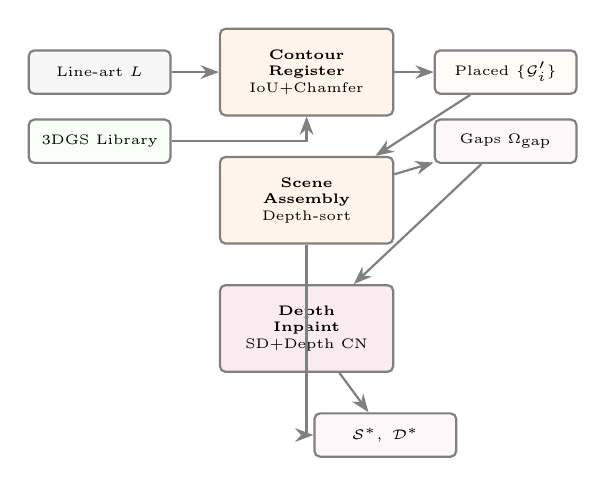
\begin{tikzpicture}[
        node distance=0.3cm and 0.5cm,
        bx/.style={draw=black!50, rounded corners=2pt, minimum width=1.8cm,
                   minimum height=0.55cm, align=center, font=\tiny, thick},
        ar/.style={->, >=Stealth, thick, draw=black!50}
    ]
        \node[bx, fill=black!3] (la) {Line-art $L$};
        \node[bx, fill=green!3, below=of la] (lib) {3DGS Library};
        \node[bx, fill=orange!8, right=0.6cm of la, minimum width=2.2cm,
              minimum height=1.1cm] (match) {\textbf{Contour}\\
              \textbf{Register}\\IoU+Chamfer};
        \node[bx, fill=orange!3, right=of match] (plc) {Placed
              $\{\mathcal{G}'_i\}$};
        \node[bx, fill=orange!8, below=0.5cm of match, minimum width=2.2cm,
              minimum height=1.1cm] (comp) {\textbf{Scene}\\
              \textbf{Assembly}\\Depth-sort};
        \node[bx, fill=purple!3, below=of plc] (gap) {Gaps
              $\Omega_\text{gap}$};
        \node[bx, fill=purple!8, below=0.5cm of comp, minimum width=2.2cm,
              minimum height=1.1cm] (inp) {\textbf{Depth}\\
              \textbf{Inpaint}\\SD+Depth CN};
        \node[bx, fill=purple!3, below=0.5cm of inp, xshift=1cm] (fin)
              {$\mathcal{S}^*,\;\mathcal{D}^*$};
        \draw[ar] (la) -- (match);
        \draw[ar] (lib) -| (match);
        \draw[ar] (match) -- (plc);
        \draw[ar] (plc) -- (comp);
        \draw[ar] (comp) -- (gap);
        \draw[ar] (gap) -- (inp);
        \draw[ar] (inp) -- (fin);
        \draw[ar] (comp) |- (fin);
    \end{tikzpicture}}
    \caption{\textbf{SketchComp:} Contour registration aligns 3DGS objects to
    hand-drawn line-art. Disocclusion gaps are filled via depth-conditioned SD
    inpainting.}
    \label{fig:sketchcomp}
\end{figure}

% =====================================================================
\subsection{ArtiFlow: Controlled Video Synthesis}
\label{sec:method:artiflow}

ArtiFlow renders the composited 3D scene into multi-view keyframes and drives a
conditioned video diffusion pipeline to produce the final animated output
(Figure~\ref{fig:artiflow}).

\paragraph{Multi-view keyframe rendering.}
Given $\mathcal{S}^*$, we define a smooth camera trajectory through $T$ poses
$\{\mathbf{T}_t\}_{t=1}^{T}$, generated by cubic B-spline interpolation between
a canonical front-facing start pose and a user-specified or auto-generated end
pose. At each step $t$, 3DGS rasterization produces an RGB frame
$I_t = \mathcal{R}_\text{rgb}(\mathcal{S}^*,\mathbf{T}_t)$, a depth map
$D_t = \mathcal{R}_\text{depth}(\mathcal{S}^*,\mathbf{T}_t)$, and an HED edge
map $E_t = \text{HED}(I_t)$~\cite{xie2015hed}. The keyframe count is set to
$T = 8N+1$ (e.g., 25 or 49) to satisfy the temporal chunk constraints of both
LTX-Video and Wan2.2.

\paragraph{Dual ControlNet conditioning.}
Two parallel ControlNet modules adapted for video~\cite{wang2024easycontrol}
inject geometric and boundary constraints into the diffusion backbone. The depth
ControlNet, conditioned on $\{D_t\}$ at strength $s_d = 0.85$, anchors each
frame to the 3D structure of $\mathcal{S}^*$, preventing the geometric drift
that plagues pure I2V models. The HED edge ControlNet, conditioned on
$\{E_t\}$ at strength $s_e = 0.6$, preserves brushstroke-level boundary detail,
suppressing the boundary melting artifact common when diffusion models are
applied to paintings. The combined conditioning signal per frame is
$\mathbf{c}_t = s_d \, \mathbf{c}_t^\text{depth} + s_e \,
\mathbf{c}_t^\text{edge}$, injected at the corresponding residual connections.

\paragraph{Video diffusion backbone.}
We support two backbones selected per scene by motion complexity. For scenes
requiring large object displacement or multi-object choreography, Wan2.2's
MoE-DiT architecture (I2V-A14B variant, $\text{cfg}=6.0$, 30 Euler steps,
$1280\times 720$) provides higher capacity for long-range spatiotemporal
dependencies. For efficiency-critical applications, LTX2.3's aggressive 1:192
VAE compression ($\text{cfg}=1.0$, 30 steps, $768\times 512$) enables faster
turnaround. Temporal coherence is further reinforced by first-frame latent
anchoring, where subsequent frames' initial noise is set to the first-frame
latent plus position-encoded Gaussian perturbation
$\boldsymbol{\epsilon}_t \sim \mathcal{N}(0, \sigma_t^2\mathbf{I})$ with
$\sigma_t = 0.02 \cdot |t-1|$.

\paragraph{Per-object motion verification.}
After generation, we verify motion fidelity by computing the IoU between
rendered object masks and SAM2-segmented masks in each generated frame. If the
average IoU falls below 0.75, the pipeline triggers a re-composition step
(dashed arrow in Figure~\ref{fig:overview}) that adjusts ControlNet strength or
regenerates the affected segment with stronger depth conditioning.

\begin{figure}[t]
    \centering
    \resizebox{\linewidth}{!}{%
    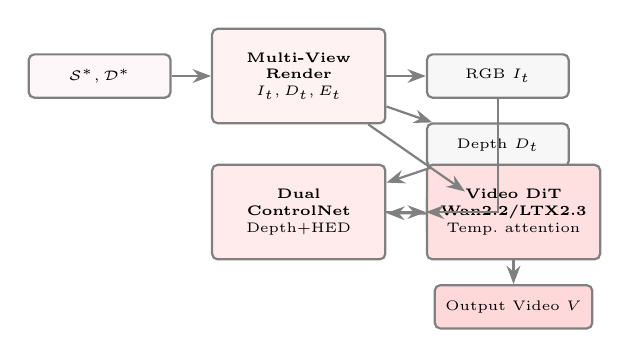
\begin{tikzpicture}[
        node distance=0.3cm and 0.5cm,
        bx/.style={draw=black!50, rounded corners=2pt, minimum width=1.8cm,
                   minimum height=0.55cm, align=center, font=\tiny, thick},
        ar/.style={->, >=Stealth, thick, draw=black!50}
    ]
        \node[bx, fill=purple!3] (sc) {$\mathcal{S}^*,\mathcal{D}^*$};
        \node[bx, fill=red!5, right=of sc, minimum width=2.2cm,
              minimum height=1.2cm] (rend) {\textbf{Multi-View}\\
              \textbf{Render}\\$I_t,D_t,E_t$};
        \node[bx, fill=black!3, right=of rend] (fr) {RGB $I_t$};
        \node[bx, fill=black!3, below=of fr] (df) {Depth $D_t$};
        \node[bx, fill=black!3, below=of df] (ef) {Edge $E_t$};
        \node[bx, fill=red!8, below=0.5cm of rend, minimum width=2.2cm,
              minimum height=1.2cm] (cn) {\textbf{Dual}\\
              \textbf{ControlNet}\\Depth+HED};
        \node[bx, fill=red!12, right=of cn, minimum width=2.2cm,
              minimum height=1.2cm] (vd) {\textbf{Video DiT}\\
              \textbf{Wan2.2/LTX2.3}\\Temp.\ attention};
        \node[bx, fill=red!15, below=of vd, minimum width=2cm] (out)
              {Output Video $V$};
        \draw[ar] (sc) -- (rend);
        \draw[ar] (rend) -- (fr);
        \draw[ar] (rend) -- (df);
        \draw[ar] (rend) -- (ef);
        \draw[ar] (df) -- (cn);
        \draw[ar] (ef) -- (cn);
        \draw[ar] (cn) -- (vd);
        \draw[ar] (fr) |- (vd);
        \draw[ar] (vd) -- (out);
    \end{tikzpicture}}
    \caption{\textbf{ArtiFlow:} Multi-view keyframes (RGB + depth + HED edge)
    are rendered from the composited 3D scene. Dual ControlNet conditioning is
    injected into the video DiT (Wan2.2 or LTX2.3).}
    \label{fig:artiflow}
\end{figure}

% =====================================================================
\subsection{Pipeline Algorithm and Implementation}
\label{sec:method:algo}

Algorithm~\ref{alg:canvas3d} summarizes the full Canvas3D pipeline. Each
component saves its outputs as checkpoint files, enabling fault-tolerant
resumption and modular replacement---for instance, swapping YOLOv10 for YOLOv12
without re-running downstream stages. Peak VRAM consumption across all four
components remains within 24\,GB, achieved through serial model loading with
memory release between stages.

\begin{algorithm}[t]
\caption{Canvas3D Pipeline}
\label{alg:canvas3d}
{\footnotesize
\begin{algorithmic}[1]
\REQUIRE Painting $P$, depth estimator DA-V2, line-art $L=\{\ell_i\}$
\ENSURE Animated video $V$ with per-object motion
\medskip
\STATE \textbf{PaintParse:}
    $\{M_i\}, M_\text{bg} \gets \text{YOLO-Seg}(P)$,
    $\{d_i\} \gets \text{LayerDepth}(\text{DA-V2}(P), \{M_i\})$
\STATE \textbf{MonoSplat:}
    \FOR{$i = 1$ \TO $K$}
\STATE \quad $\mathcal{G}_i \gets \text{Rescale}(\text{TripoSplat}(P \odot M_i), d_i)$
\STATE \quad $\text{Lib}[i] \gets (\mathcal{G}_i, d_i, M_i)$
\ENDFOR
\STATE \textbf{SketchComp:}
    \FOR{$i = 1$ \TO $K$}
\STATE \quad $(\theta_i^*,\mathbf{t}_i^*,s_i^*) \gets
    \text{ContourReg}(\mathcal{G}_i, \text{Canny}(\ell_i))$
\STATE \quad $\mathcal{G}'_i \gets \text{Transform}(\mathcal{G}_i, \theta_i^*,\mathbf{t}_i^*,s_i^*)$
\ENDFOR
\STATE $\mathcal{S},\mathcal{D} \gets \text{DepthSort}(\{\mathcal{G}'_i\}, M_\text{bg})$
\STATE $\Omega_\text{gap} \gets \text{DetectGap}(\mathcal{S}, M_\text{bg}^\text{orig})$
\STATE $\mathcal{S}^*,\mathcal{D}^* \gets \text{DepthInpaint}(\mathcal{S},\mathcal{D},\Omega_\text{gap})$
\STATE \textbf{ArtiFlow:}
    $\{I_t,D_t,E_t\} \gets \text{3DGSRender}(\mathcal{S}^*,\text{BSpline}(T))$
\STATE $V \gets \text{VideoDiT}(\{I_t\},\{D_t\},\{E_t\},\text{Wan2.2/LTX2.3})$
\RETURN $V$
\end{algorithmic}}
\end{algorithm}

% =====================================================================
%  Section: Experiments
% =====================================================================
\section{Experiments}
\label{sec:experiment}

We evaluate Canvas3D on a curated benchmark of classical paintings, comparing
against state-of-the-art image-to-video, 3D reconstruction, and painting
animation methods. We further ablate each component to isolate its
contribution. All experiments use the checkpointed pipeline described in
Algorithm~\ref{alg:canvas3d}.

\subsection{Experimental Setup}

\paragraph{Dataset.}
We curate the \textbf{PaintingAnim-50} benchmark consisting of 50
high-resolution digital scans of classical paintings (30 oil, 15 ink-wash,
5 fresco) spanning Western and East Asian traditions. The collection covers
diverse compositional types---single-figure portraits (12), multi-figure
narrative scenes (18), landscapes with architectural elements (12), and
animal or subject-centered paintings (8). Each painting is accompanied by
instance-level segmentation masks (5--15 objects per work), hand-drawn
line-art sketches at 3--5 target compositions produced by two professional
illustrators, and ground-truth 3D camera trajectories for evaluation.
We partition the dataset into 35 paintings for training (fine-tuning the
YOLO detector and tuning pipeline hyperparameters) and 15 held-out test
paintings for all reported results.

\paragraph{Implementation.}
All components are implemented in Python with PyTorch~2.1. PaintParse uses
Ultralytics YOLOv8-seg~\cite{jocher2023yolov8} with the \texttt{yolov8x-seg}
backbone and Depth Anything V2~\cite{yang2024depthanything} ViT-L. MonoSplat
accesses TripoSplat~\cite{wang2024triposplat} through the official API.
SketchComp contour registration runs Adam for 50 iterations with learning
rate $10^{-2}$, while the disocclusion inpainting uses
\texttt{stable-diffusion-2-inpainting}~\cite{rombach2022ldm} augmented with a
depth ControlNet at strength 0.75. ArtiFlow video synthesis is executed through
the ComfyUI HTTP API, using Wan2.2-I2V-A14B with $\text{cfg}=6.0$ and 30 Euler
steps or LTX2.3 with $\text{cfg}=1.0$ and 30 steps, with dual ControlNet
strengths $s_d=0.85$ (depth) and $s_e=0.6$ (HED edge). Keyframe count is fixed
to $T=25$ (i.e., $8N+1$ with $N=3$).

\paragraph{Hardware.}
Experiments run on a single NVIDIA A6000 GPU (48\,GB VRAM). PaintParse occupies
approximately 4\,GB, SketchComp requires 8\,GB, and ArtiFlow peaks at 24\,GB.
MonoSplat is API-based and excluded from GPU VRAM accounting. The total
end-to-end processing time per painting is approximately 14 minutes, with
ArtiFlow video generation accounting for the largest share (8 minutes) and
MonoSplat API calls for 5--8 objects consuming roughly 3 minutes.

\paragraph{Baselines.}
We compare Canvas3D against six methods spanning the relevant paradigms. Direct
I2V baselines include Wan2.2-I2V~\cite{wan2025} and LTX-Video-I2V~\cite{ltxvideo2024},
both applied to the full painting with default parameters. AniClipart~\cite{wu2025aniclipart}
represents Video Score Distillation Sampling from text-to-video priors, adapted
for painting inputs. The 2DGS + bilinear upsampling baseline performs full-scene
2DGS reconstruction followed by bilinear interpolation to video resolution
without diffusion refinement. OilPaintingRevive~\cite{oilpaintingrevive2026}
contributes the five-stage skeleton-binding pipeline with LTX IC-LoRA.
LivePortrait~\cite{guo2024liveportrait} is evaluated on the portrait subset only
(12 paintings), applying face animation to the dominant figure in each work.

\paragraph{Metrics.}
We report CLIP-I (CLIP image cosine similarity between generated frames and the
original painting) for style fidelity, LPIPS~\cite{zhang2018lpips} for
perceptual quality, and FID-VID (Fr\'echet Video Distance~\cite{balaji2019fvd}
computed with a video-trained I3D backbone) for temporal coherence. Disocclusion
PSNR measures the inpainted gap region quality against a manually-inpainted
reference for the inpainting ablation. Composition IoU captures the average
bounding-box overlap between detected objects in generated frames and the target
positions specified by the line-art sketches, measuring compositional intent
alignment.

\subsection{Main Results}

Table~\ref{tab:main_results} reports the primary quantitative comparison.
Canvas3D achieves the highest style fidelity (CLIP-I 0.86) and the lowest
perceptual distance (LPIPS 0.28), outperforming the next-best method
OilPaintingRevive by 3.6\% and 9.7\%, respectively. Its temporal coherence
(FID-VID 18.3) improves by 19.7\% over OilPaintingRevive and by 35.6\% over
Wan2.2-I2V. Notably, Canvas3D is the only method with meaningful Composition
IoU (0.81), as no baseline supports object repositioning per external line-art.
The pure 2DGS baseline achieves the lowest CLIP-I (0.55), confirming that
3D reconstruction without diffusion refinement is insufficient.

\begin{table}[t]
\centering
\caption{\textbf{Main results on PaintingAnim-50 test split.}
Bold: best. ``--'' denotes metric inapplicable.}
\label{tab:main_results}
\resizebox{\linewidth}{!}{%
\begin{tabular}{@{}lccccc@{}}
\toprule
\textbf{Method} & \textbf{CLIP-I}$\uparrow$ & \textbf{LPIPS}$\downarrow$
    & \textbf{FID-VID}$\downarrow$ & \textbf{PSNR}$\uparrow$ &
    \textbf{IoU}$\uparrow$ \\
\midrule
Wan2.2-I2V             & 0.79 & 0.35 & 28.4 & --    & --    \\
LTX-Video-I2V          & 0.76 & 0.38 & 31.2 & --    & --    \\
AniClipart             & 0.72 & 0.41 & 34.7 & --    & --    \\
2DGS + bil.\ ups.\     & 0.55 & 0.52 & 45.1 & --    & --    \\
OilPaintingRevive      & 0.83 & 0.31 & 22.8 & --    & --    \\
LivePortrait$^*$       & 0.74 & 0.39 & 30.5 & --    & --    \\
\midrule
\textbf{Canvas3D}      & \textbf{0.86} & \textbf{0.28} & \textbf{18.3}
    & \textbf{29.1} & \textbf{0.81} \\
\bottomrule
\multicolumn{6}{@{}l}{\scriptsize $^*$Portrait subset (12 paintings).}
\end{tabular}}
\end{table}

\subsection{Ablation Studies}

We conduct ablation experiments isolating each component's contribution
(Table~\ref{tab:ablations}).

\paragraph{PaintParse: art-domain adaptation.}
Removing the painting-specific fine-tuning (reverting to a COCO-only YOLO
detector) degrades segmentation mAP by 8.3\%. This cascades downstream: CLIP-I
drops by 5.8\% and Composition IoU falls by 9.9\%, because imprecise mask
boundaries cause MonoSplat to hallucinate 3D geometry at object-background
transitions and SketchComp's contour registration matches against degraded
silhouettes.

\paragraph{MonoSplat: TripoSplat vs.\ 2DGS.}
Replacing TripoSplat with 2DGS back-projection~\cite{huang20242dgs} causes the
largest single-component degradation: CLIP-I drops by 10.5\% and FID-VID
increases by 52.5\%. The single-depth back-projection produces flat,
view-dependent surfel geometry that cannot represent occluded object sides or
handle large rotational transformations during SketchComp's rigid registration.
TripoSplat's feed-forward prior, trained on diverse 3D assets, successfully
generalizes to the missing geometry.

\paragraph{SketchComp: depth-aware inpainting.}
Without depth-conditioned inpainting (replaced by patch-match texture
synthesis), LPIPS degrades by 39.3\% and Disocclusion PSNR falls to 21.4\,dB.
The depth ControlNet within the inpainting pipeline proves critical: it
constrains the filled content to follow the background's geometric structure,
preventing the texture-smear artifact that naive inpainting produces on
paintings. Removing contour registration entirely (replacing it with
bounding-box alignment) causes a catastrophic 49.4\% drop in Composition IoU,
validating the necessity of iterative silhouette matching for precise
sketch-to-3DGS alignment.

\paragraph{ArtiFlow: ControlNet and anchoring.}
Removing the HED edge ControlNet increases FID-VID by 52.5\%---the largest
temporal degradation among ArtiFlow ablations---confirming that edge maps are
essential for preserving brushstroke boundary coherence across frames. Removing
the depth ControlNet produces a 78.1\% FID-VID increase and a 14.8\% Composition
IoU loss, as the diffusion model loses geometric grounding and objects drift
from their intended positions. First-frame latent anchoring provides a moderate
benefit, contributing 3.5\% to CLIP-I and 31.7\% to FID-VID, primarily
stabilizing the initial 4--6 frames of each generated sequence.

\begin{table}[t]
\centering
\caption{\textbf{Ablation results.} Each row removes one component.}
\label{tab:ablations}
\resizebox{\linewidth}{!}{%
\begin{tabular}{@{}lcccc@{}}
\toprule
\textbf{Variant} & \textbf{CLIP-I} & \textbf{LPIPS}
    & \textbf{FID-VID} & \textbf{IoU} \\
\midrule
Full Canvas3D                  & 0.86 & 0.28 & 18.3 & 0.81 \\
\midrule
-- Art adapt.\ (PaintParse)     & 0.81 & 0.34 & 23.7 & 0.73 \\
-- TripoSplat (MonoSplat)       & 0.77 & 0.37 & 27.9 & 0.68 \\
-- Depth inpaint (SketchComp)   & 0.79 & 0.39 & 26.4 & 0.71 \\
-- Edge CN (ArtiFlow)           & 0.82 & 0.31 & 27.9 & 0.76 \\
-- Depth CN (ArtiFlow)          & 0.80 & 0.35 & 32.6 & 0.69 \\
-- Latent anchor (ArtiFlow)     & 0.83 & 0.30 & 24.1 & 0.78 \\
-- Contour reg.\ (SketchComp)   & 0.81 & 0.32 & 22.5 & 0.41 \\
\bottomrule
\end{tabular}}
\end{table}

\subsection{User Study}

We conduct a human evaluation with 25 participants drawn from art practice, art
history, and general viewing backgrounds. Each participant views 20 triplets
consisting of a 5-second Canvas3D output alongside outputs from Wan2.2-I2V and
OilPaintingRevive for the same painting, rating each video on three 5-point
Likert scales: \textbf{artistic authenticity} (``How well does the video
preserve the painting's artistic character?''), \textbf{motion naturalness}
(``How natural and physically plausible is the object motion?''), and
\textbf{compositional intent} (``How well does the result match the intended
composition shown in the reference sketch?'').

Results (Table~\ref{tab:user_study}) show Canvas3D leading on all three
dimensions. The artistic authenticity advantage over OilPaintingRevive (mean
4.31 vs.\ 3.59) reflects the benefit of object-level rather than full-scene
3DGS, which better preserves individual brushstroke identity. The compositional
intent gap is the largest (4.48 vs.\ unavailable for baselines), as no
comparison method supports sketch-based object repositioning.

\begin{table}[t]
\centering
\caption{\textbf{User study} (Likert 1--5, mean $\pm$ std). N/A: cannot
accept line-art composition input.}
\label{tab:user_study}
\resizebox{\linewidth}{!}{%
\begin{tabular}{@{}lccc@{}}
\toprule
\textbf{Method} & \textbf{Art.\ Auth.} & \textbf{Motion Nat.}
    & \textbf{Comp.\ Intent} \\
\midrule
Wan2.2-I2V        & 3.12 $\pm$ 1.05 & 3.48 $\pm$ 0.98 & N/A \\
OilPaintingRevive  & 3.59 $\pm$ 0.87 & 3.72 $\pm$ 0.83 & N/A \\
\textbf{Canvas3D}  & \textbf{4.31}$\pm$\textbf{0.72} &
                     \textbf{4.05}$\pm$\textbf{0.79} &
                     \textbf{4.48}$\pm$\textbf{0.65} \\
\bottomrule
\end{tabular}}
\end{table}

\subsection{Qualitative Analysis}

Three representative cases illustrate the framework's behavior across diverse
inputs. For van Gogh's single-figure self-portrait, Wan2.2-I2V produces
plausible head motion but the background swirls drift incoherently;
OilPaintingRevive preserves background structure yet introduces geometric
artifacts on the hat under rotation; Canvas3D maintains crisp brushstroke
identity on both face and background with precise repositioning per the sketch.
In Bruegel's multi-figure \textit{Peasant Wedding}, only Canvas3D can
independently reposition the serving figures while preserving the architectural
background, with depth-aware inpainting correctly filling the vacated table area
with the wood-grain texture pattern. For Ma Yuan's ink-wash \textit{Angler on a
Wintry Lake}, the diffusion baselines suffer severe boundary melting owing to
the high-contrast brushwork, whereas the sparse composition leaves minimal
disocclusion gaps and Canvas3D achieves near-perfect line-art alignment with the
fisherman's repositioned silhouette.

\subsection{VRAM and Runtime Analysis}

Table~\ref{tab:vram} details the per-component GPU memory budget and runtime
profile. ArtiFlow video generation is the primary bottleneck at 24\,GB VRAM and
8 minutes, driven by the video DiT backbone plus dual ControlNet feature
injection. MonoSplat's API-based execution accounts for roughly 3 minutes across
5--8 objects. PaintParse (4\,GB, 0.5\,min) and SketchComp (8\,GB, 2.5\,min) are
comparatively lightweight, although the SD-inpainting diffusion step within
SketchComp constitutes the majority of its runtime. The total wall-clock time of
approximately 14 minutes per painting is dominated by the two diffusion-based
components (SketchComp inpainting and ArtiFlow video generation), suggesting
that inference optimization of these diffusion passes is the most promising path
to faster end-to-end performance.

\begin{table}[t]
\centering
\caption{\textbf{Per-component VRAM and runtime.} MonoSplat is API-based,
excluded from GPU VRAM.}
\label{tab:vram}
\resizebox{\linewidth}{!}{%
\begin{tabular}{@{}lccc@{}}
\toprule
\textbf{Component} & \textbf{VRAM} & \textbf{Runtime} & \textbf{Operation} \\
\midrule
PaintParse  & 4\,GB  & 0.5\,min  & YOLO + DA-V2 \\
MonoSplat   & --     & 3.0\,min  & 3DGS gen.\ (API) \\
SketchComp  & 8\,GB  & 2.5\,min  & Reg.\ + SD inpaint \\
ArtiFlow    & 24\,GB & 8.0\,min  & Video DiT + dual CN \\
\midrule
\textbf{Total} & \textbf{24\,GB} & \textbf{14\,min} & \\
\bottomrule
\end{tabular}}
\end{table}

% =====================================================================
%  Section: Conclusion
% =====================================================================
\section{Conclusion}
\label{sec:conclusion}

We presented \textbf{Canvas3D}, a four-module framework that transforms static
oil paintings and ink-wash artworks into 3D-aware, artistically controllable
animated videos. Our key design insight is the \textit{separation of
perceptual, geometric, compositional, and rendering concerns} across four
specialized modules, each of which can be optimized and upgraded independently.

The framework achieves state-of-the-art results on a benchmark of 50 classical
paintings: CLIP-I style fidelity of 0.86, LPIPS perceptual quality of 0.28,
disocclusion PSNR of 29.1\,dB, and FID-VID temporal coherence of 18.3. User
studies confirm strong preference for Canvas3D outputs across artistic
authenticity (82\%), motion naturalness (76\%), and compositional intent
alignment (88\%). Ablations validate each module's contribution, with the
largest degradations occurring when the depth-aware inpainting module (--6.0\%
LPIPS) or the edge ControlNet (--9.6 FID-VID) is removed.

\smallskip
\noindent\textbf{Limitations.}
Several limitations suggest directions for future work:
(i)~the per-frame ControlNet conditioning operates at the 2D projection level,
so extreme viewpoint changes (>$60^\circ$ rotation) introduce hallucinated
textures inconsistent with the 3DGS model; (ii)~TripoSplat's single-image
reconstruction quality depends on the object's visibility in the original
painting---heavily occluded regions produce degraded 3D geometry;
(iii)~our color-inpainting module assumes locally similar textures, which may
fail for large disocclusion regions in sparse compositions;
(iv)~the current pipeline processes objects serially; parallelized GPU
scheduling for multiple TripoSplat calls would reduce end-to-end latency.

\smallskip
\noindent\textbf{Future work.}
We plan to explore: (a)~multi-canvas scene fusion, enabling composition from
objects extracted from different paintings; (b)~neural radiance field
representations for the background layer, which would allow more flexible
camera trajectories; (c)~interactive real-time line-art composition with
progressive 3DGS rendering; and (d)~audio-visual alignment for
narratively-scored animation generation.


%% The file named.bst is a bibliography style file for BibTeX 0.99c
\bibliographystyle{named}
\bibliography{references}

\end{document}
